\chapter{Image classification}
Image classification is one of the essential modern computer vision problems, where the goal is to create a model that can classify an input image into one of a set of pre-defined classes. Before the popularization of applying large Convolutional Neural Networks for this task, the most successful way of solving the problem was to use some algorithm for finding feature descriptors in a set of images to construct a Visual Bag of Words \citep{vbow}.  A linear classifier, like a Support Vector Machine, would then do the classification using the Bag of Words representation of an image. These days nearly all approaches are based on using deep CNNs, and working CNNs were deployed already in 1998 on character recognition in the form of LeNet \citep{leNet}.
In this chapter, we will present what ImageNet \citep{imagenet} is and how the models trained with it are important when applying transfer learning, and we will show an example of how it can be done.


\section{ImageNet}

ImageNet \citep{imagenet} has been one of the most significant data sets for image classification. 
It is has enabled the development and served as a benchmark for several significant improvements to modern computer vision techniques.
The ImageNet challenge \citep{ILSVRC} is a competition consisting of a selected collection of 1000 classes and a total of 1.2 million training images and 150 thousand test images from the ImageNet data set.
Winning models from the ImageNet competition have provided some of the essential architectures modern computer vision algorithms use.
In 2012 the winning model, AlexNet \citep{alexNet}, showed that it was possible to train deep CNNs efficiently using GPUs. Since 2012 all top-performing models showed some new improvements on how to create the most performant network architecture, for example, VGGNet \citep{VGG} from the year 2014 and ResNet \citep{resNet} from 2015, both of which have been popular models to use for Transfer Learning since.

Human accuracy in image classification on the ImageNet challenge is about 5.1\% \citep{imageNet_summary}, ResNet achieves a top-5 error rate of 3.57\% \citep{resNet} and newer architectures even lower, but this still does not mean that image classification is a solved problem. The human performance experiment found that many of the human errors are caused by not having expert information in, for example, identifying animal species or not even being aware of the existence of a class \citep{imageNet_summary}. ObjectNet \citep{objectNet} is a dataset designed to test image classifiers with a focus on their generalizability. It contains many classes that also exist in the ImageNet dataset. However, the objects in the images are in unexpected locations or have an unexpected pose, causing the high accuracy image classifiers trained on ImageNet to experience a 40-45\% accuracy drop when evaluating them on the ObjectNet images of classes shared between ImageNet and ObjectNet. This kind of adjustment is relatively easy for a human, and it shows that while the classifiers are good, they are by no means perfect.

\section{Transfer learning}
Transfer learning is a powerful technique to obtain results quickly when using deep CNNs. Here we will only take a look at transfer learning within the domain of deep CNNs, but it is a technique that has been successfully applied to many other domains of machine learning as well.

The idea behind transfer learning is to train on a task that would produce useful features in solving some other task. 
Then the network weights in the model for the actual task are initialized to those of the model we are transferring from, so the training of the original model is a pre-step to the real task. 
Since training the models on ImageNet scale datasets is not generally feasible due to their large number of parameters and long training time, one of the pre-trained models is picked and then fine-tuned. 
Fine-tuning a classifier means that some existing model is used as a weight initializer, and the network is then trained on the data of another task, updating the weights of the original classifier to better align with the new task. 
The transfer learning approach differs significantly from the traditional learning model, where each task requires a separate model that learns from the given data using random weights. 
Since image inputs are often very high dimensional, the traditional approach may not work in many cases. 
The pre-training allows for focusing on data that provides answers to the actual task and not on learning low-level features, which the ImageNet classifiers would already have learned.

To give a formal definition of transfer learning, we will follow the definitions provided in \citep{transferSurvey2010}. 
Let $\mathcal{D}$ be a domain, which consists of a feature space $\mathcal{X}$ and a marginal probability distribution P($\mathcal{X}$). 
For a given domain, a task $\mathcal{T}$ \[\mathcal{T} = \{\mathcal{Y}, f\mathcal(X)\}\] \noindent consists of a label space $\mathcal{Y}$ for the inputs and of a predictive function $f(x)$ which produces predictions for all pairs \{$x_i, y_i$\} where $x_i \in \mathcal{X}$ and $y_i \in \mathcal{Y}$. 
Given a source domain $\mathcal{D}_S$, a source task $\mathcal{T}_S$, a target domain $\mathcal{D}_T$ and a target task $\mathcal{T}_T$, where target and source are disjoint, transfer learning tries to improve the performance of $f_T(x)$ using $\mathcal{D}_S$ and $\mathcal{T}_S$.

Unlike the ImageNet challenge, most real-world tasks do not have such an abundance of data for all possible classes. Still, to achieve the highest accuracies, they require models that are equal in terms of complexity to those that have top accuracies problems on the scale of the ImageNet classification. For this reason, many CNN classifiers, irrespective of the problem, feature one of the ImageNet classifiers in the model architecture. Even though some datasets may contain a large number of images per class, using a pre-trained classifier as a basis often produces a better final classifier by applying fine-tuning \citep{betterTransfer}.

\begin{figure}[h!] 
\centering 
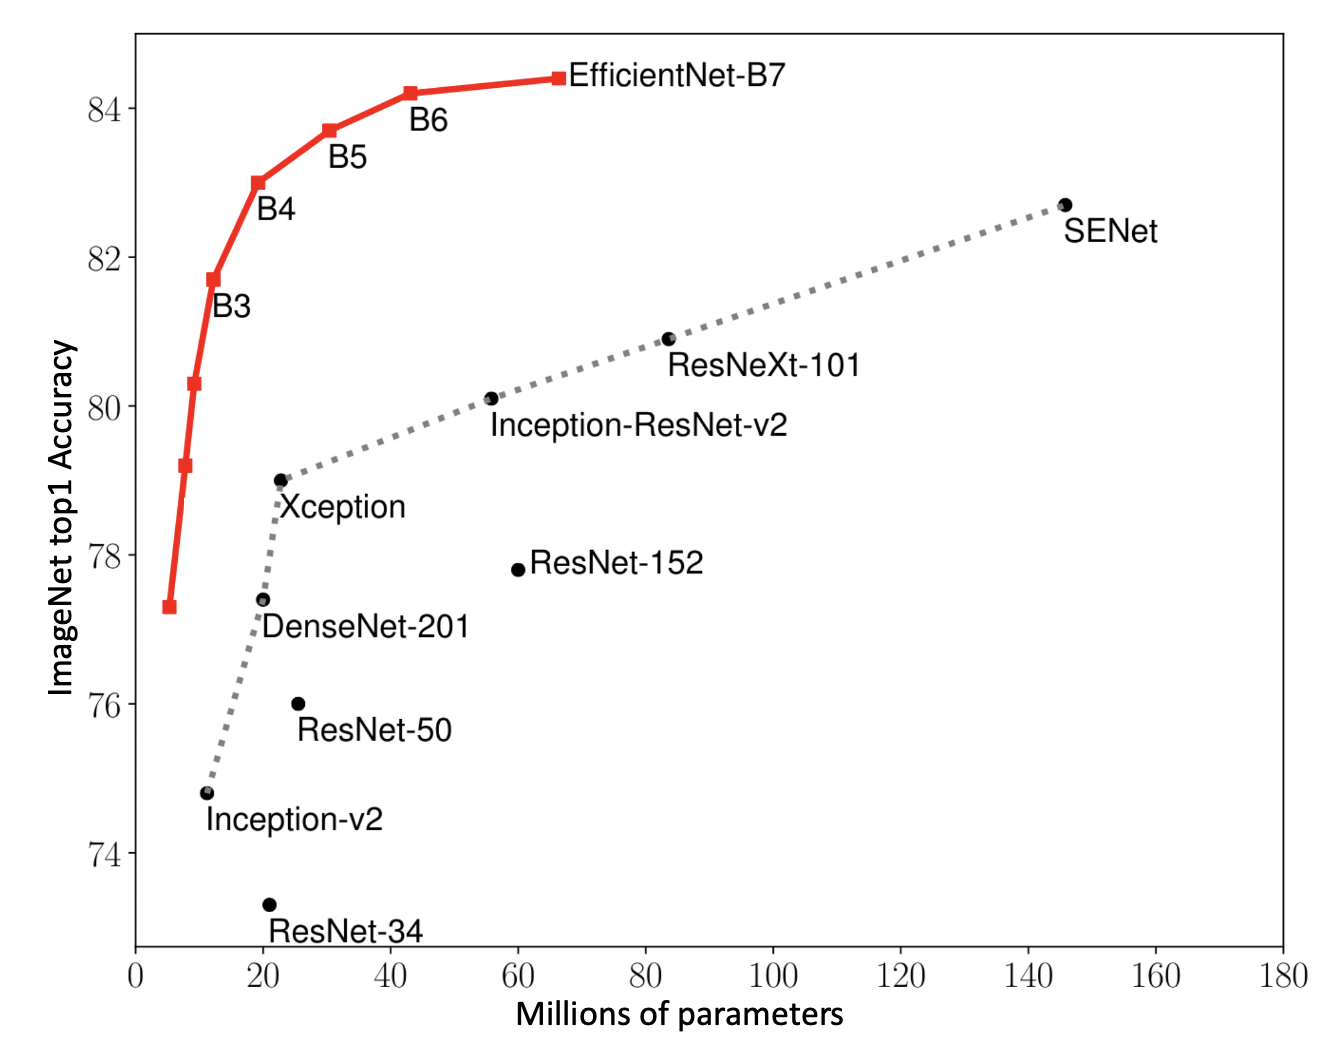
\includegraphics[width=0.8\textwidth]{imgs/imagenet-own.png}
\caption{Number of parameters in popular ImageNet classifiers. Figure adapted from \citep{efficientNet}.\label{fig:params}}
\end{figure}

Picking which classifier to use as a base is often problem-dependent. As it is not possible to declare one network structure to be the best at all tasks, picking the best model to start with usually requires the user to compare different architectures and weighing the requirements for the problem at hand. Often though, the larger models will perform better, and there exists a correlation between performing well on ImageNet and being a good transfer learning model \citep{betterTransfer}. Though as can be seen in figure 3.1, better performance often comes at the cost of many more parameters, requiring more memory to train the model. Though, as the results in \citep{classifierPerformance} show, just the number of parameters is not the only thing to compare as the throughput of a Resnet50 turns out to be about three times as large as the throughput of an EfficientNet-B4 \citep{efficientNet} even though they have a similar amount of parameters. So in the case of time-constrained inference environments, also the time required for an inference has to be taken into account when picking models.
Often though, the number of parameters is a relatively good proxy for the inference time.
The throughput is likely due to the differences in the internal implementations of the EfficientNet and normal CNNs.

If there is enough data, it turns out that using a pre-trained network does not provide any benefits in terms of the converged model accuracy, but it is not detrimental to performance either \citep{rethinkTransfer}. When training sufficiently long on a sufficient amount of data, the pre-trained and randomly initialized networks converged to similar accuracies but required significantly different amounts of training resources. Still, this does not mean that pre-training is useless by any means as the saved resources and getting models to converge faster are essential factors for progress. And of course, there is not enough data in many cases, and training from scratch will not provide satisfying results due to the large number of parameters that would need to be optimized.
In these cases, it would then be a decision to apply transfer learning or to get a model that is not good enough to produce reliable results.

\section{ResNet}
ResNet is one of the first effective and very deep Convolutional Neural Network architecture that was presented in 2015 and won the ImageNet challenge. Prior to the publication of ResNet, the most powerful networks were relatively shallow, like VGGNet \citep{VGG}, which has only 19 layers. One of the big issues relating to training deep networks is vanishing gradients, where gradients disappear when they are backpropagated through many layers \citep{wideResNet}. ResNets utilize residual connections around bottleneck building blocks, which allow for the networks to contain many more layers than those without them, the largest network presented in the original ResNet paper was 152 layers, totaling for around 8x increase in the number of layers when compared to earlier networks \citep{resNet}.

\begin{figure}[h!] 
\centering 
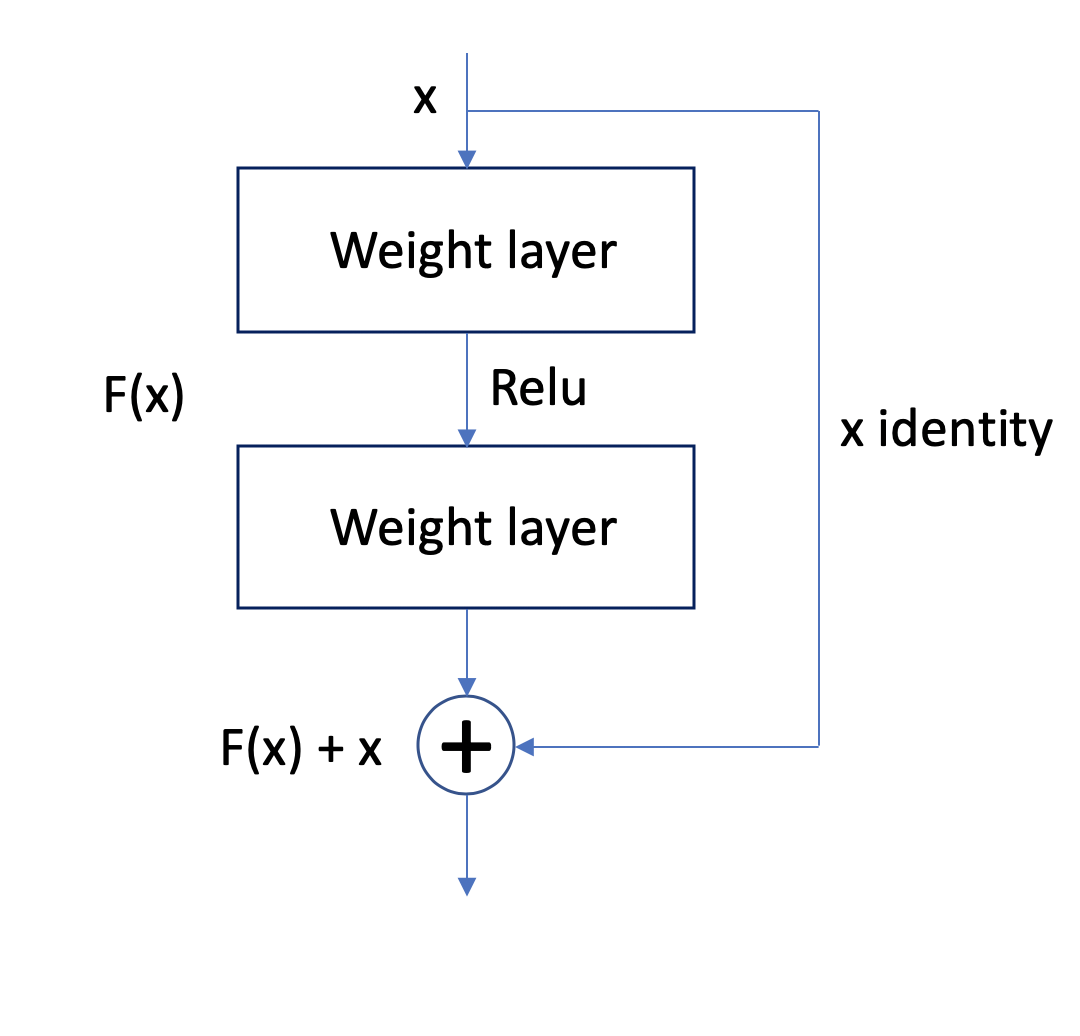
\includegraphics[width=0.8\textwidth]{imgs/resnet-block-own.png}
\caption{Resnet building block for learning the residual \citep{resNet}}
\end{figure}

The ResNet block architecture allows for the blocks to learn the identity function more efficiently by trying to learn the residual function instead of the direct mapping. The residual can be learned by adding the unchanged weights of an earlier layer to the output of some transformations on it.
The residual block is shown in Figure 3.2.
Normally a neural network layer learns the mapping between ${x}$ and ${y}$ using a function ${H(x)}$, but by the same token, we can learn a residual transformation.
Learning these residuals using the identity mapping skip-connections is the revolutionary idea introduced by the ResNet.
Since these skip-connections are only connections and not extra layers, they do not require extra parameters that would need to be learned.
The residual transformation is
\[{F(x) = H(x) - x}\] \noindent where ${H}$ is the mapping of two or more network layers. Both of these approaches should approximate the same functions; the difference is in how easy it is for the network to learn. Learning a transformation of ${F(x) = 0}$ would intuitively seem easier for a neural network than learning ${F(x) = x}$. As can be seen from the success of the ResNets compared to non-residual networks, this is what allows for creating very deep networks. If the transformation changes the input size, a matrix ${W}$ is necessary to map the input to the same dimensions, generating the final formula for a residual block. \[y = F(x, \{W_i\}) + W_s x\] \noindent where $W_i$ and $W_s$ are the the weight matrices to be applied to x.

Many variants of ResNet exists, such as wide ResNets \citep{wideResNet}, ResNeXt \citep{resNext} and others. Also the DenseNet \citep{denseNet} is heavily inspired by ResNets. ResNet-50, ResNet-34, ResNet-101, and ResNet-152 are still some of the most popular models to use when a pre-trained ImageNet trained backbone is needed for some part of a classifier as they produce good results and do not contain too many parameters compared to some other architectures.

\section{Improving model performance}
Improving model performance is not easy, but using the various types of skip-connections, such as the ones used in ResNet residual blocks with the identity transform, it is possible to increase the size of the network to massive sizes. A 557 million parameter model called GPipe \citep{gPipe} takes the model scaling to the extreme and requires some unique parallelism libraries to train the model. It is still only slightly better than previous models, showing that size is not the only thing that matters.

\begin{figure}[h!] 
\centering 
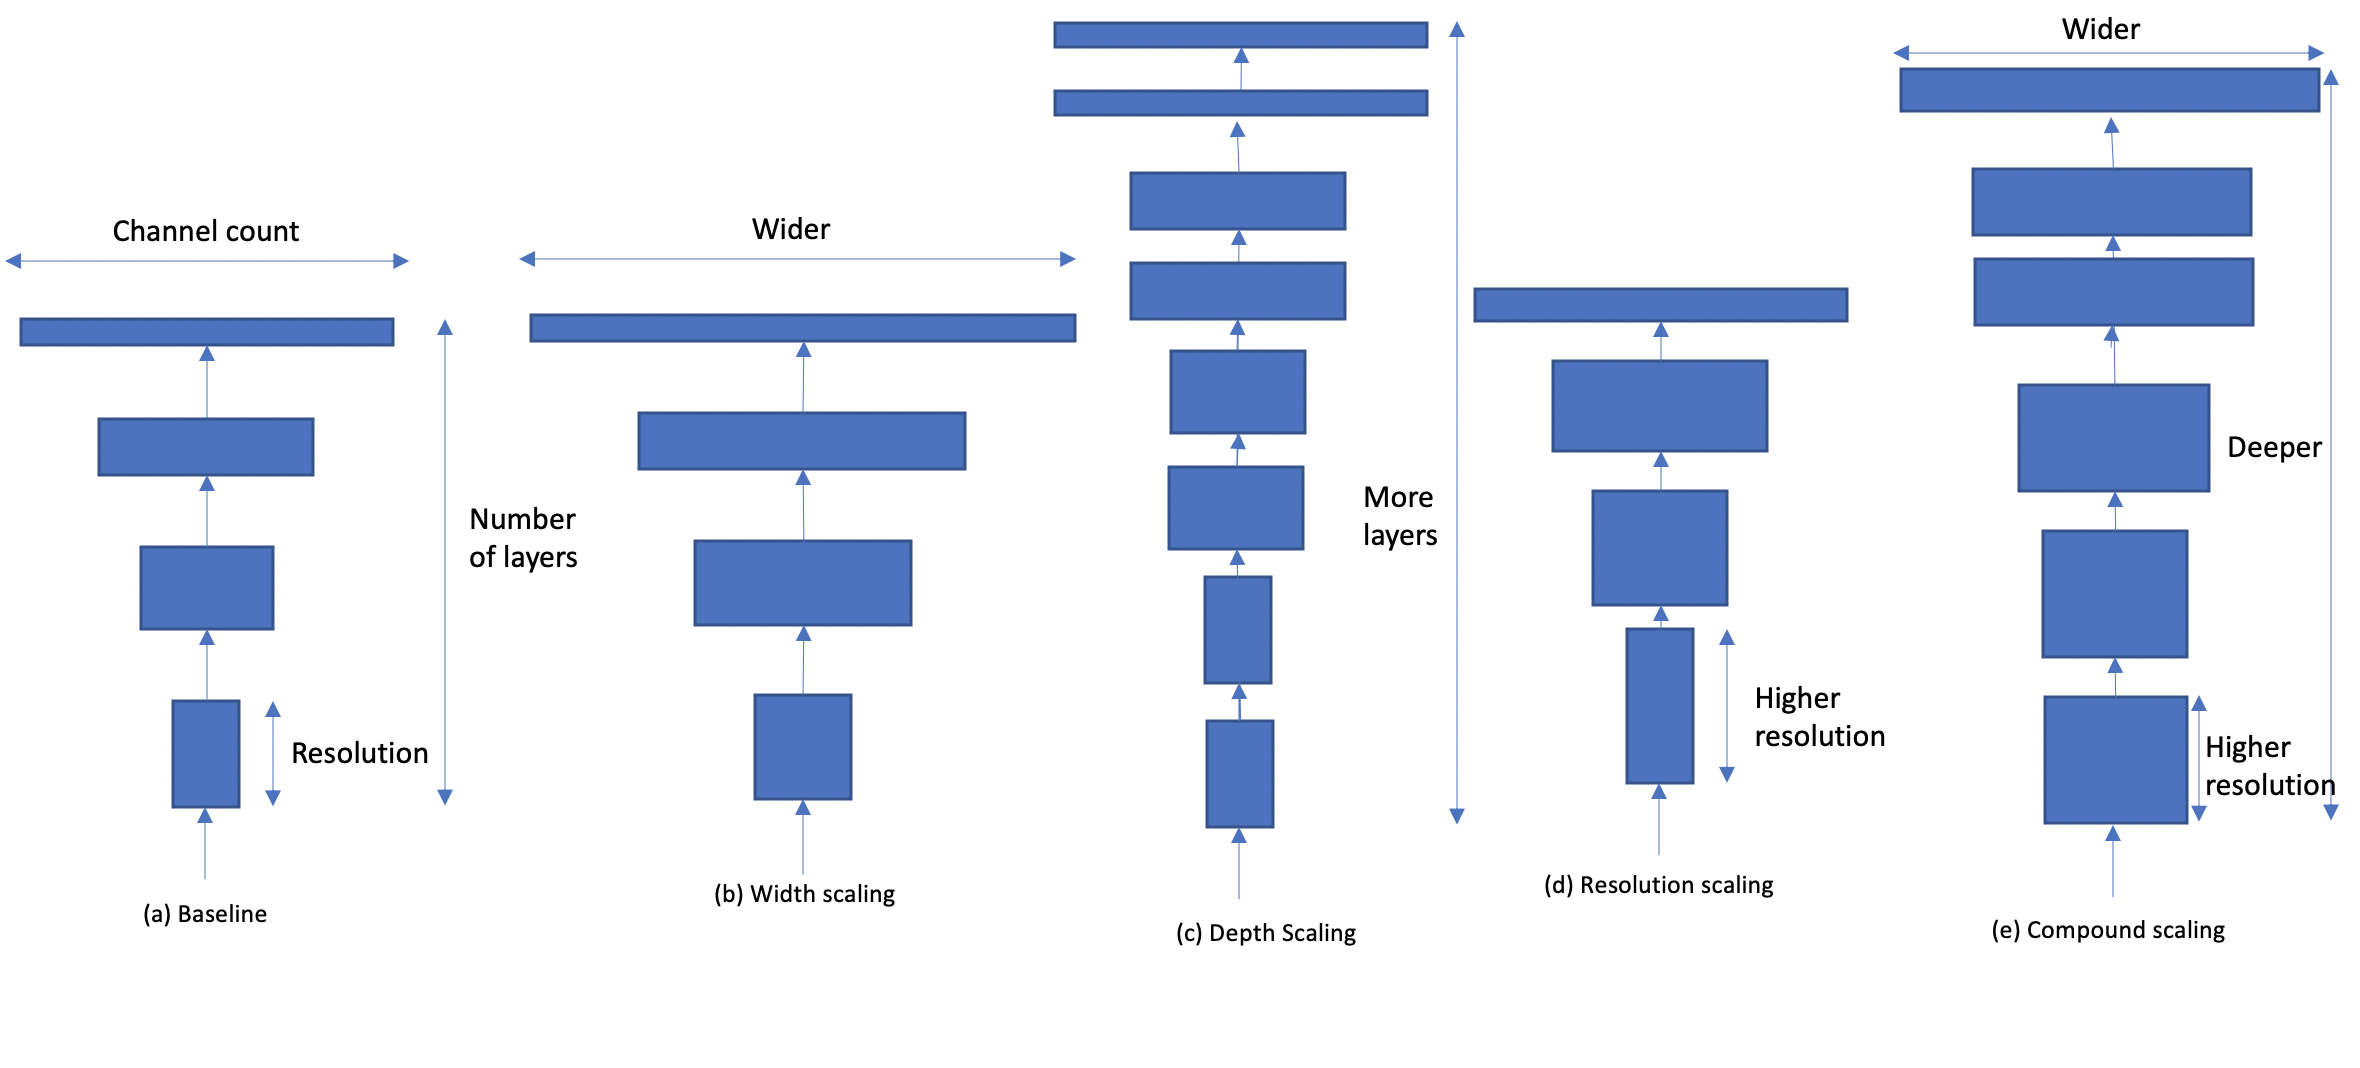
\includegraphics[width=0.8\textwidth]{imgs/scaling-networks-own.png}
\caption{Various ways of scaling network architectures \citep{efficientNet}. a) Shows the baseline network. b) Shows how to scale by the number of channels. c) Shows how to scale the number of layers. d) Shows how to scale by resolution. e) Shows how to scale all the metrics with a compound factor.}
\end{figure}

There are three main ways to scale up a network, as shown in figure 3.3. Scaling by depth means adding more layers to the model, allowing for more complex dependencies to be captured by the model. For example, ResNet-1000 is a very deep type of ResNet, but it has similar performance to a ResNet-101, so there are diminishing returns when trying to scale up by depth \citep{efficientNet}. Scaling by width means increasing the number of channels in the layers, and it is especially popular when optimizing smaller size models, such as MobileNet \citep{mobileNet}. Wide ResNets \citep{wideResNet} increase the width of the ResNet blocks and allow for better features and easier training. The third way is to increase the resolution of the input. A higher resolution allows for the network to find more specific features as the level of detail increases, and often specific network architectures work best at one particular resolution.

The other approach to finding a better architecture is to use different kinds of blocks that are better. One way of finding better building blocks is by manual experimentation. The other, like in the case of MnasNet \citep{mnas}, is to pose the problem as an optimization problem and to use Neural Architecture Search \citep{neuralSearch} to find the optimal solution. In the case of MnasNet, the goal is to maximize the model architecture m in \[ACC(m) \times [\frac{LAT(m)}{T}]^w \] \noindent where ${T}$ is the target, by searching in a constrained space. So the goal is to optimize the accuracy (ACC) of the model with a given latency (LAT) on a specific device. The search produces small but very efficient models when the target device is a mobile phone.

\section{EfficientNet}
EfficientNet models form a family of models ranging from EfficientNet0 to EfficientNet7 that were generated by smartly scaling existing convolutional models to optimize them for efficiency in a similar way to MnasNet \citep{efficientNet}. 
The more complex models are created by using compound scaling on the EfficientNet0 model, shown in Figure 3.3 (e),  where the width, depth, and the resolution of the network are scaled using a factor ${\phi}$. 
As the cost of neural architecture search grows exponentially as the size of the network grows, the search is only done on the base model. 
The search of ${\phi}$ is a constrained optimization problem, where width, depth and, resolution are constrained such that ${d^\phi \times w^\phi \times r^\phi \approx 2}$ and each increase in ${\phi}$ increases network FLOPS by ${2^\phi}$. 
The architecture search for the base network is similar to that of MnasNet. The target of EfficinetNet is to maximize the model m  \[ACC(m) \times [\frac{FLOPS(m)}{T}]^w\] \noindent so the goal is to optimize for both accuracy (ACC) and number of floating-point operations (FLOPS) instead of latency as in MnasNet \citep{efficientNet}. 

As seen in figure 3.1, these optimizations allow for the EfficientNet to form a very performant architecture using a low amount of parameters that does well on ImageNet and is good at Transfer Learning also. Interestingly though, the reduction in FLOPS and parameters do not directly translate to low real-world inference time. As is compared in the paper, an EfficientNet-B1 gets a 5.7x speedup over a ResNet-152, while the EfficientNet scores significantly higher on ImageNet. So in terms of the time and accuracy ratio, the EfficientNet seems to do well. When looking at the inference time in terms of FLOPS and parameters, we can find out that the ResNet would be more efficient, as the ResNet has 7.6x as many parameters and 16x FLOPS when compared to the EfficientNet, but the inference time multiplier is 5.7x. From this comparison, we can easily see that the number of FLOPS is not a direct proxy for inference time. 
Instead, the optimization should be for latency directly as in MnasNet if that is the goal.

The proposed EfficientNet models use mobile inverted bottleneck (MBConv) blocks used in MobileNetV2 \citep{mobileNetv2} in constructing the base model. The MobileNet uses a Depthwise Separable Convolution, where a depthwise convolution and a pointwise convolution are applied in sequence. The depthwise convolution applies ${d_i}$ ${k x k}$ filters to the input, where ${d_i}$ is the input channels and ${k}$ is the kernel size leading to an output channel count ${d_j = d_i}$. A normal convolutional layer would apply multiple filters having ${M}$ channels with the computational cost of ${h_i w_i d_i d_j k^2}$, whereas the depthwise convolution only has a cost of ${h_i w_i d_i (k^2 + d_j)}$, reducing the cost by ${k^2}$. The result of the depthwise convolution then runs through a pointwise convolution, where a ${1 \times 1 \times d_j}$ 1d convolution is applied to get the final output as a linear combination of the channels. The inverted residuals in MBConv are connections similar to ResNet, but in this case, they are connected between the low dimensional layers.

\section{Training image classifiers}
An image classifier's basic function is to predict which of some set of classes exists in an image.
So, to train a model to answer such a question, a data set with images and accompanying labels are needed.
For example, the Oxford-IIT Pets dataset \citep{catsdogs} consists of images of 37 different cat and dog species and labels for those images signifying which of the 37 classes an image represents.
The dataset consists of about 200 images per class, so it is relatively small and an excellent example of a situation where transfer learning is instrumental in getting good results.

After the data of the images and labels are gathered to a data loader, that outputs small batches for training, the model needs to be constructed.
For the backbone, any ImageNet classifier will do. 
For example, EfficientNet-B4 could be a good decision.
So we will initialize the backbone of our model with the weights of a pre-trained EfficientNet that was trained on the ImageNet data set by someone with access to large computational resources.
After the model has been initialized, the head has to be changed to be compatible with our new task.
By default, the model will be expecting to classify images to the thousand classes of the ImageNet.
In this case, we want to solve the 37 cat and dog species problem, so the final fully connected layer has to be changed.
It will be initialized as a fully connected layer with 37 output units, representing each of the classes, connecting the embedding to the outputs.
The head does not need to be just a single, fully connected layer, but it could also contain more fully connected layers, dropout layers, and batch normalization layers and more.
Adding more than a single fully connected layer might be a good idea if the backbone remains frozen and is not fine-tuned. 
That way, the head can learn some useful combinations of the image embedding instead of optimizing the features in the backbone.

Once all the layers are in place, the model needs to be optimized with a training loop.
Every iteration, a loss needs to be calculated for the batch that has been sampled from the data loader.
To be able to calculate the loss, the outputs of the final fully connected layer need to be normalized into a distribution of probabilities with softmax.
The softmax is defined as
\[{Softmax(x_i) = \frac{exp(x_i)}{\sum_j exp(x_j)}}\] \noindent
For each class $i$, there is an output score of $x_i$, for which we will calculate the proportion of its score with respect to the sum of all the classes' scores $x_j$, creating the probability distribution.
Since we have a single correct class, we would want to maximize the probability of the correct class and minimize the probability of the other classes.
The loss function to do exactly this optimization is called categorical cross-entropy, and it is defined as follows.
\[{CE = -\frac{1}{N}\sum_{i=1}^{N}(y_i * log(p_i) + ( 1 - y_i ) * log ( 1 - p_i))}\] \noindent
Where $N$ is the number of classes, $y_i$ is either 1 or 0 depending on if it is the correct label and $p_i$ is the probability for that class.
This formula does exactly what we previously described that we wanted to do.
To get the loss for a single class, if $y = 1$, the value will be the first part of the sum, if $y = 0$, the value will be the second part of the sum, since $(1 - y_i)$ is now 1.
When we optimize the model, in the case of the chosen architecture, the model will reach around 95\% accuracy on this data set \citep{efficientNet}.